
%\section{PD Klassendiagramm}

%\begin{figure}[H]
%  \begin{center}
    %{\rotatebox{90}{\includegraphics[height=...cm]{./images/...}}}
%  \end{center}
%  \caption{Klassendiagramm PD}
%\end{figure}


\section{PD Klassendiagramm}

\begin{figure}[H]
  \begin{center}
    {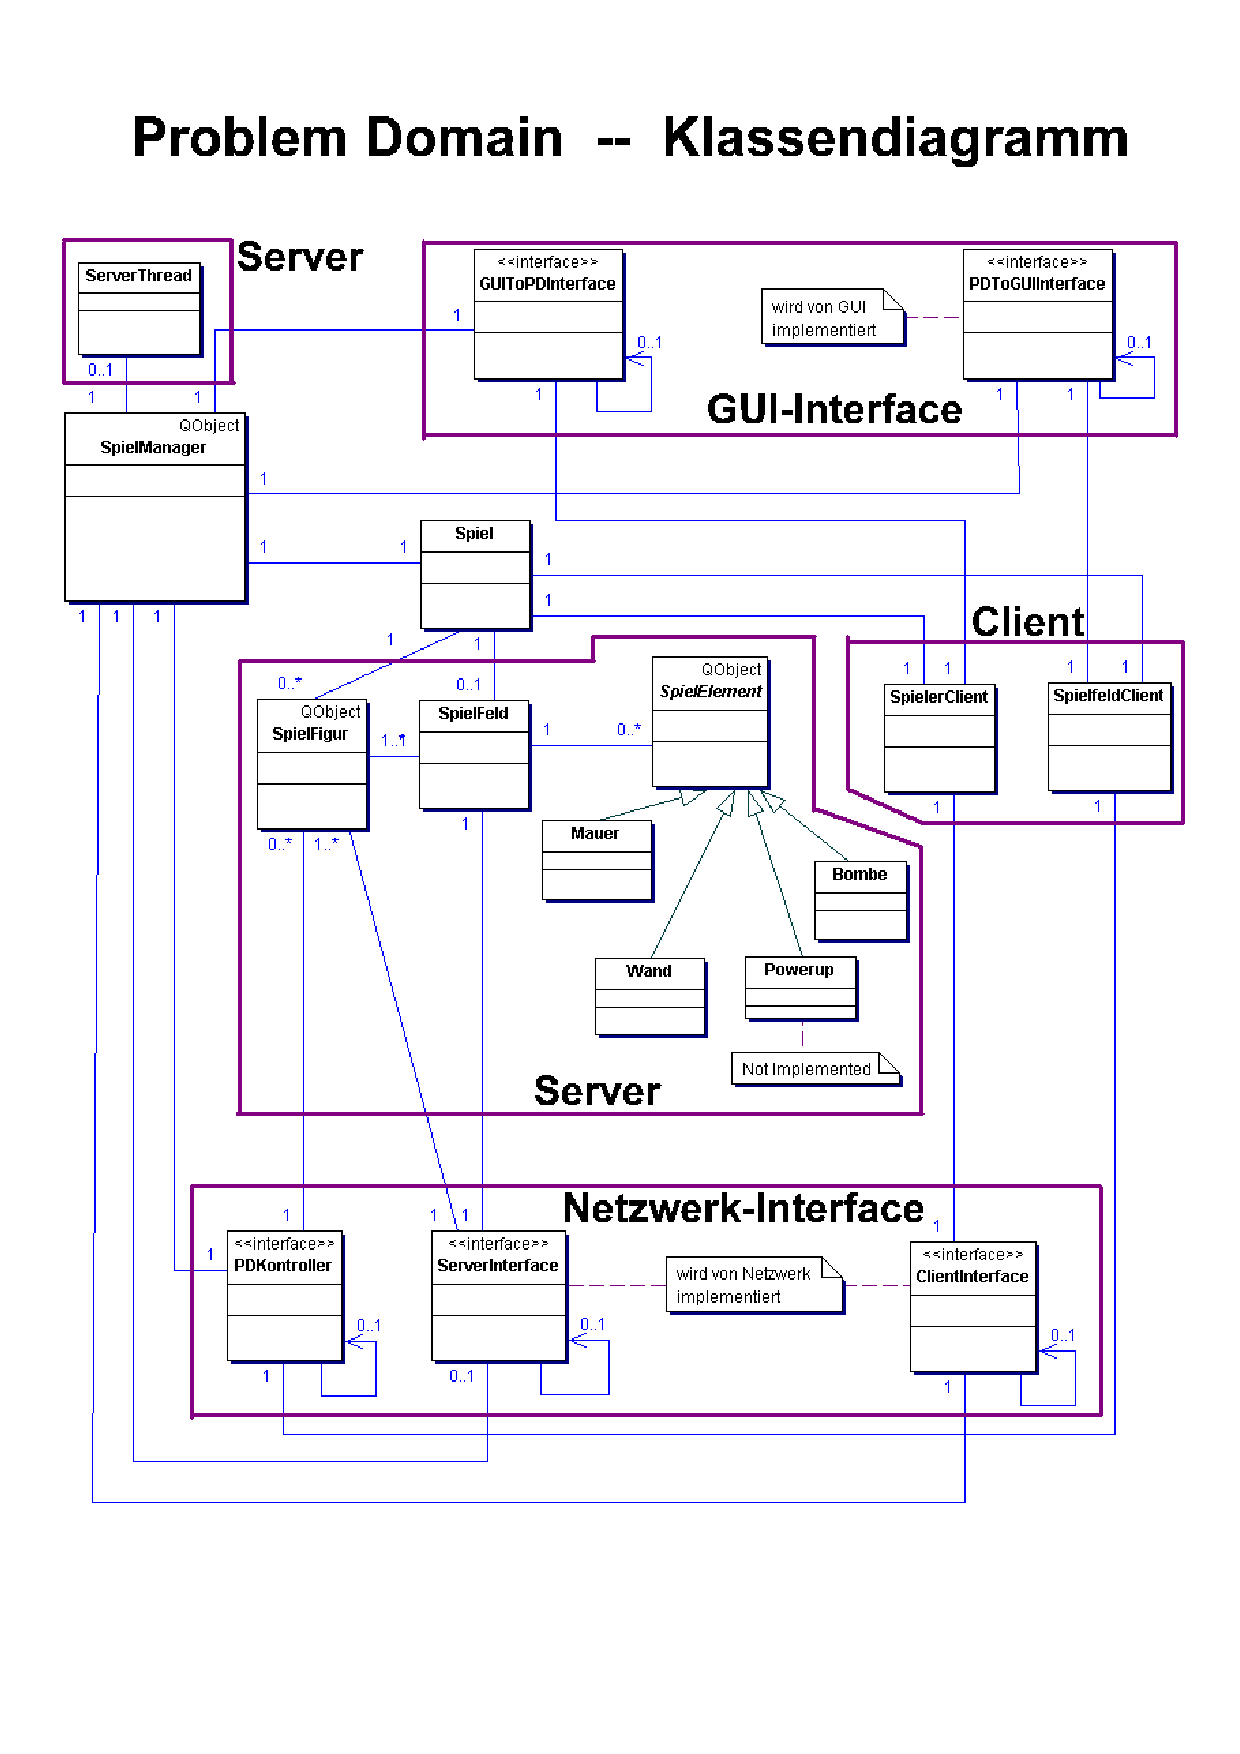
\includegraphics[height=18cm]{./images/pda4g.pdf}}
  \end{center}
  \caption{Klassendiagramm PD (siehe auch A3 Blatt in Register 9)}
\end{figure}

\section{PD Sequenzdiagramme}

\begin{figure}[H]
  \begin{center}
    {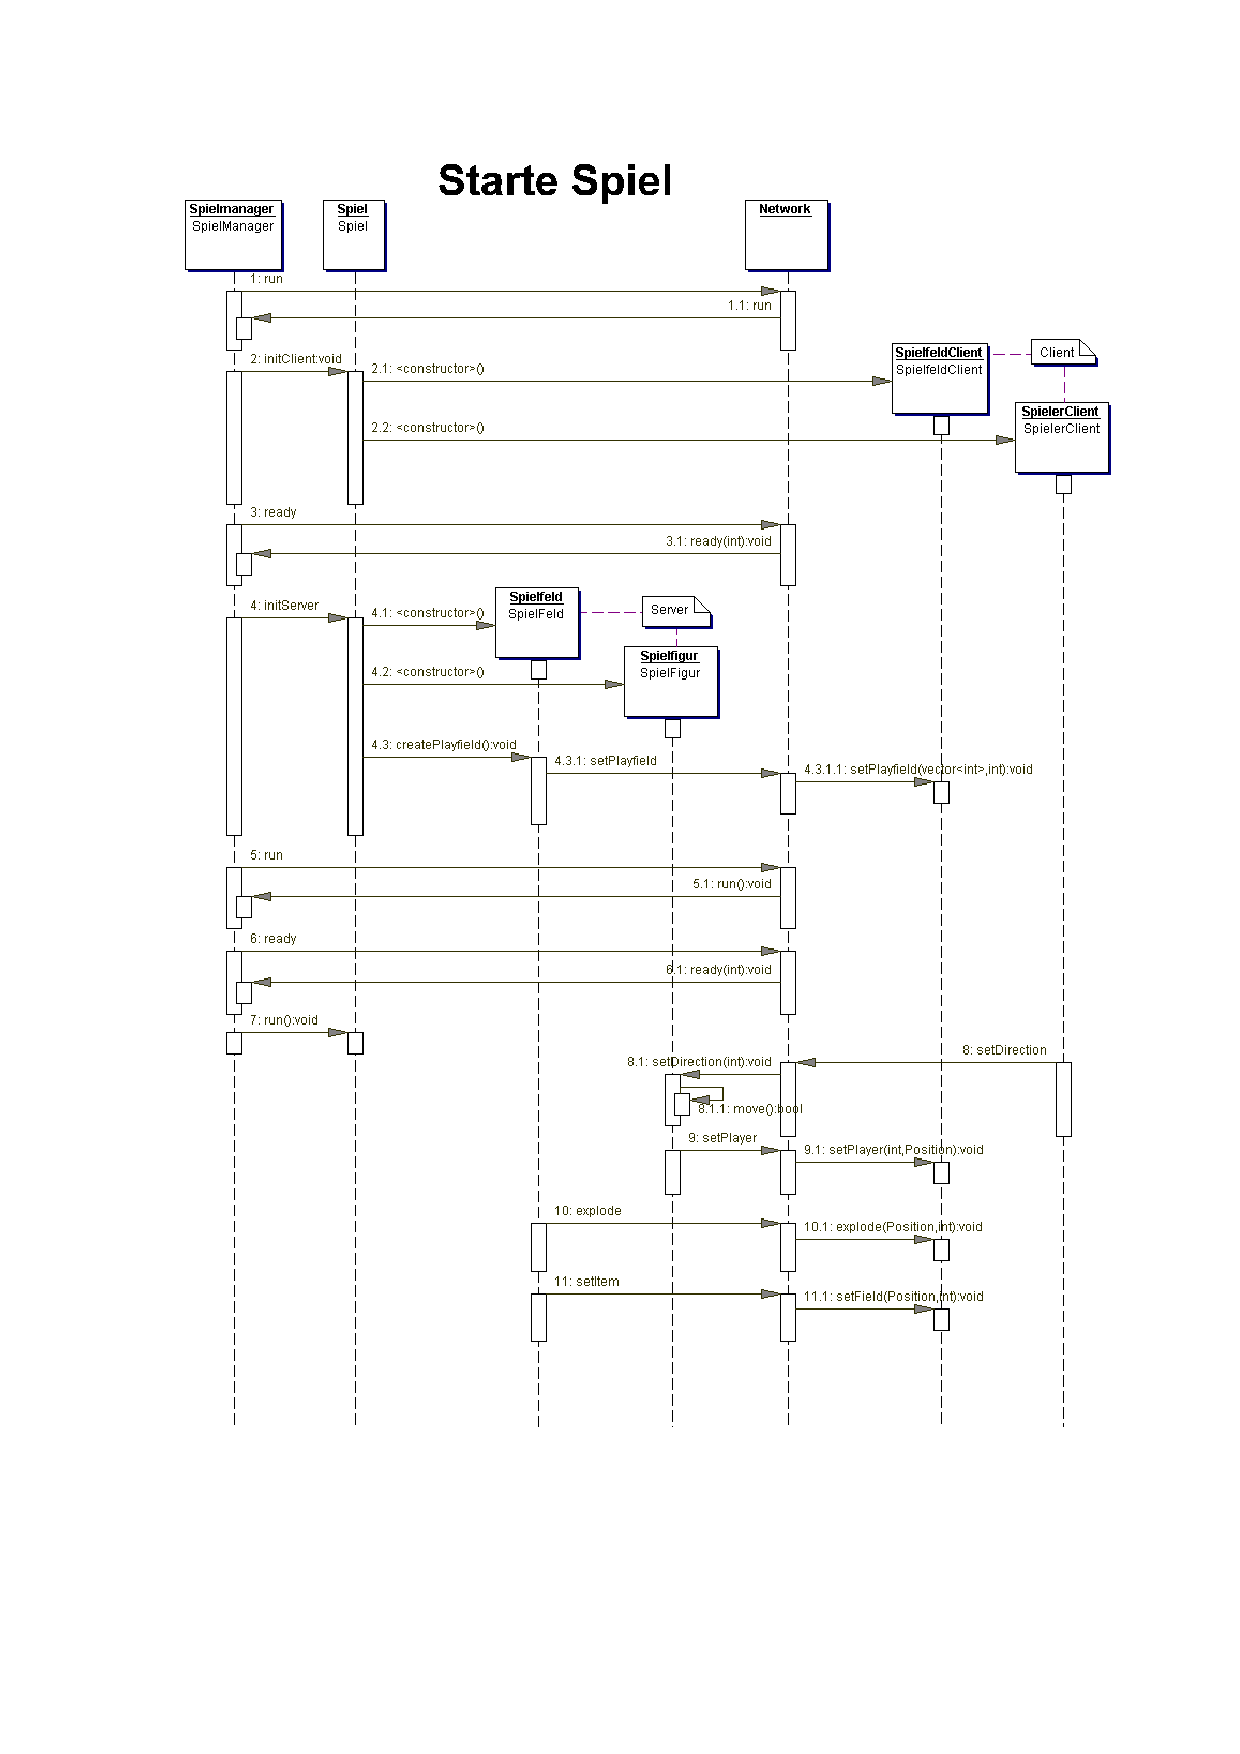
\includegraphics[height=18cm]{./images/startespiel2.pdf}}
  \end{center}
  \caption{Sequenzdiagramm f"ur neues Spiel}
\end{figure}

\begin{figure}[H]
  \begin{center}
    {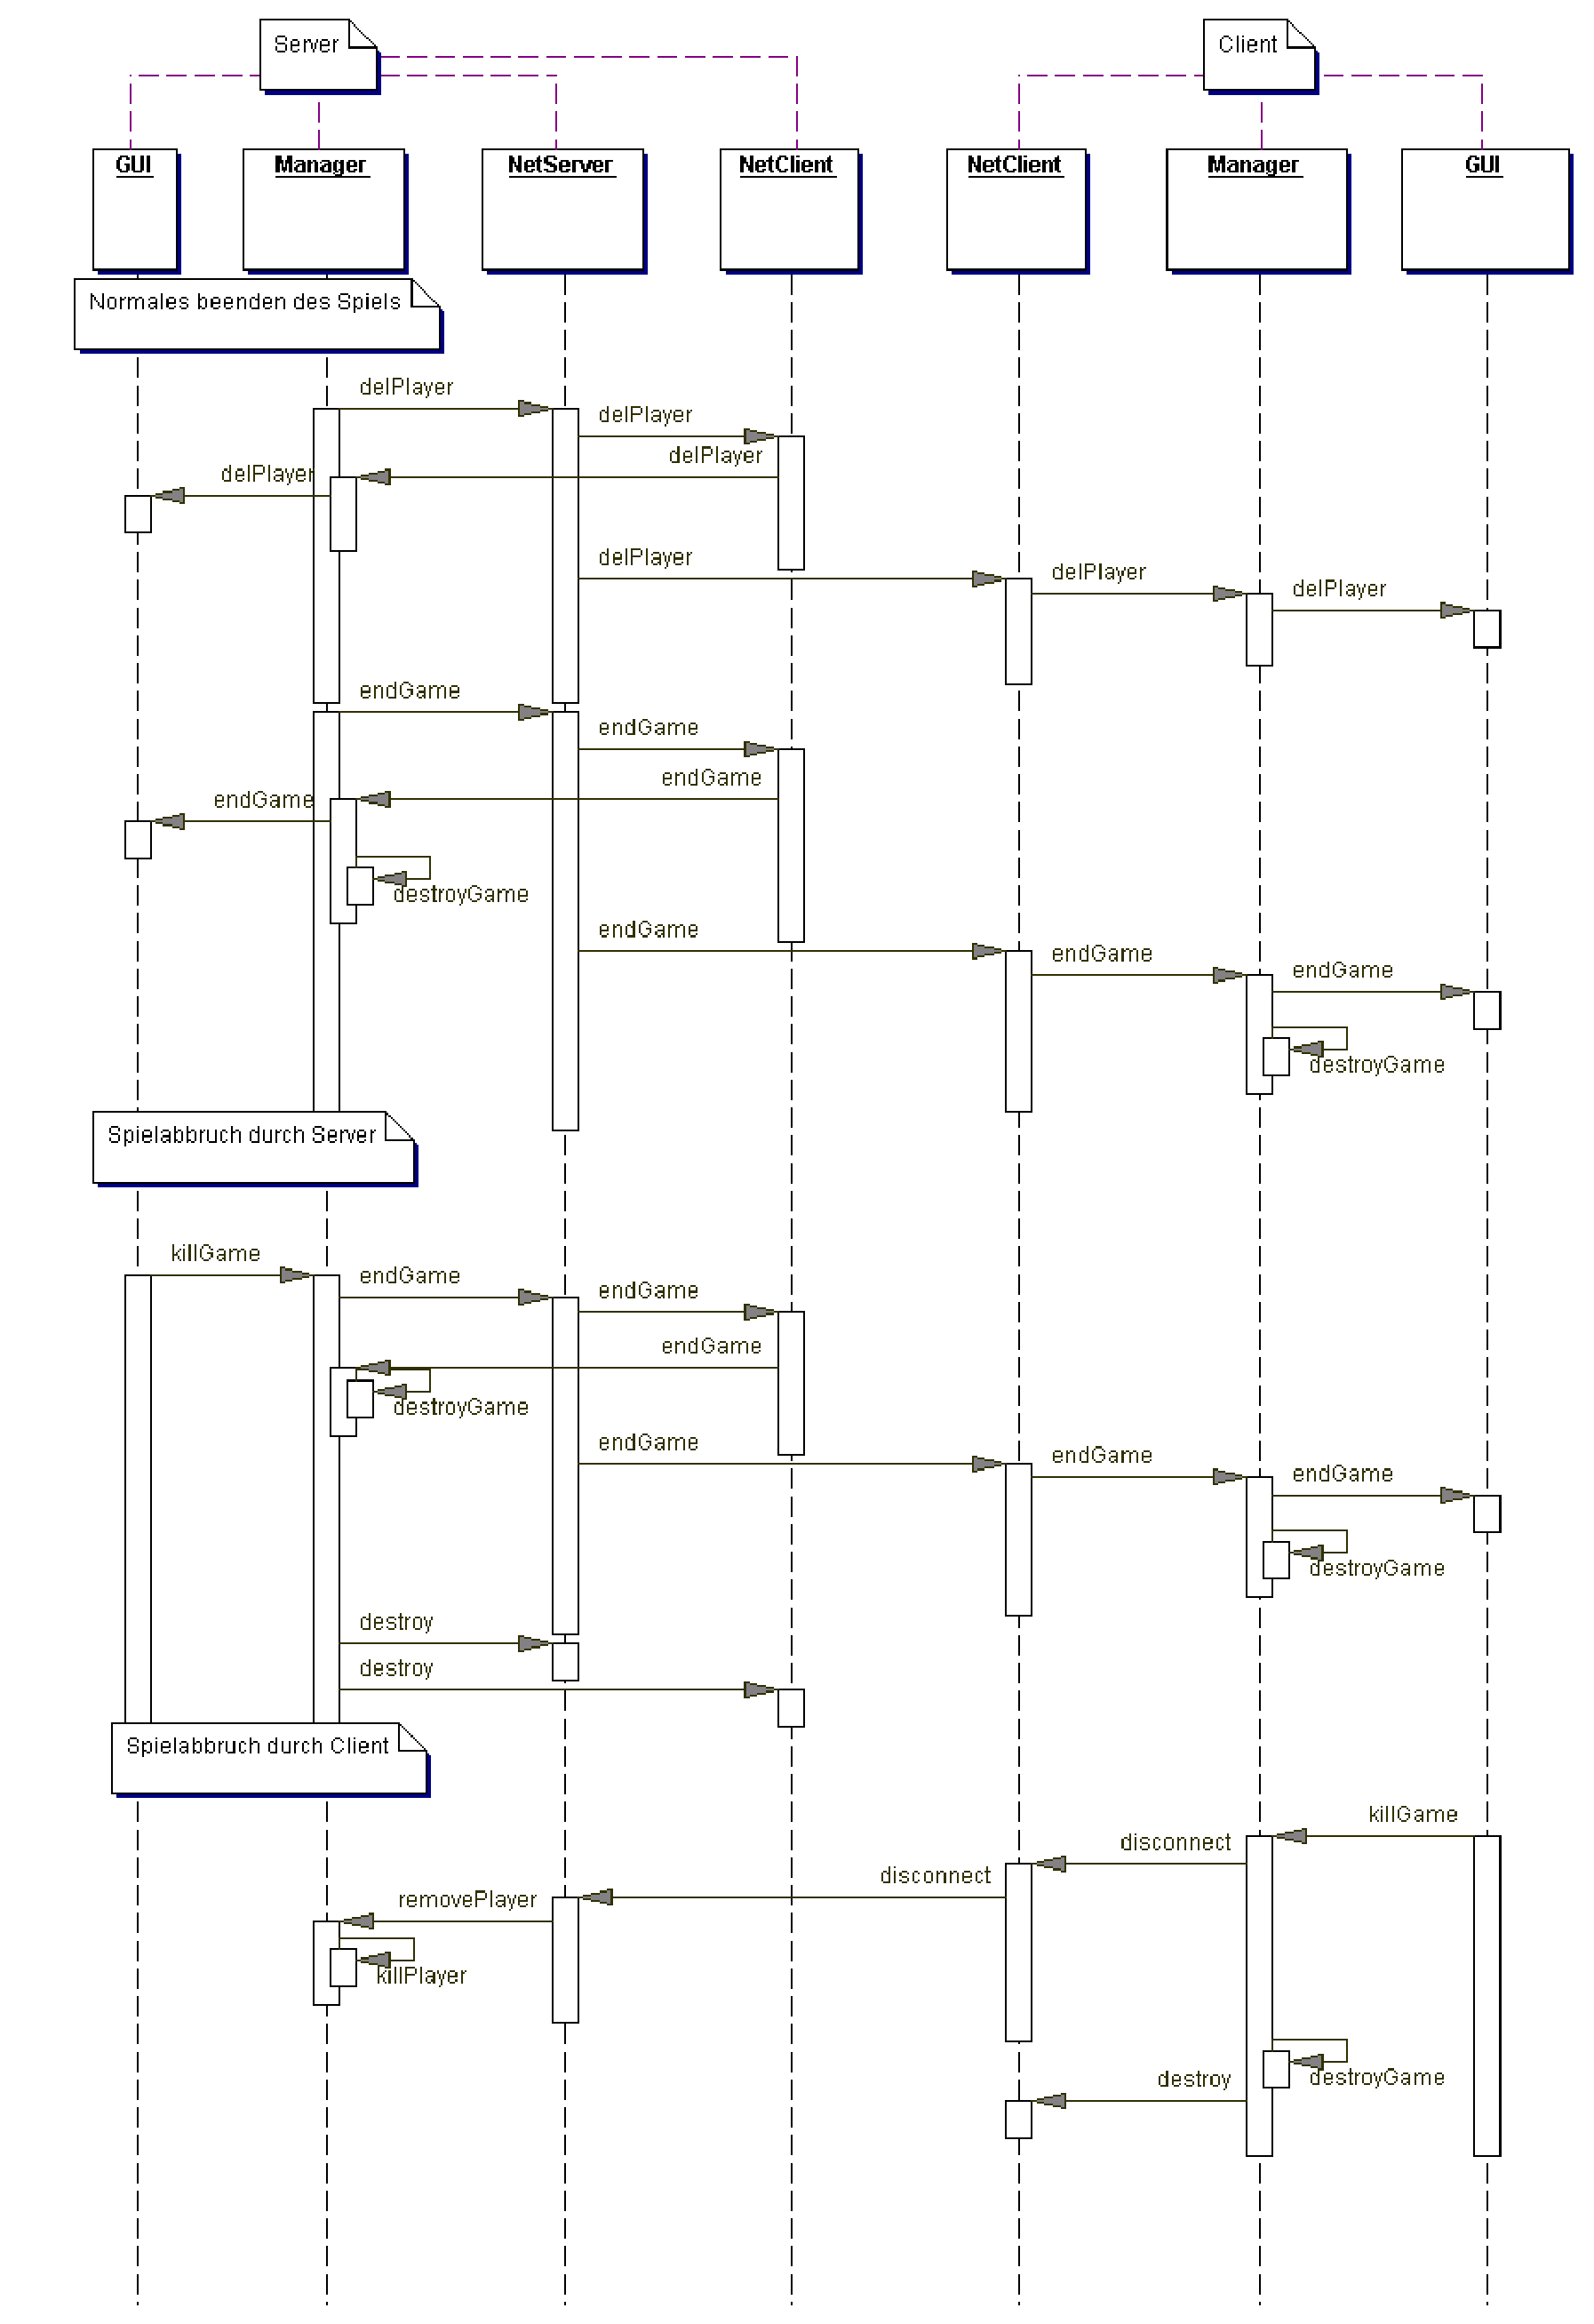
\includegraphics[height=18cm]{./images/endgame.pdf}}
  \end{center}
  \caption{Sequenzdiagramm f"ur das Beenden des Spiels}
\end{figure}

\begin{figure}[H]
  \begin{center}
    {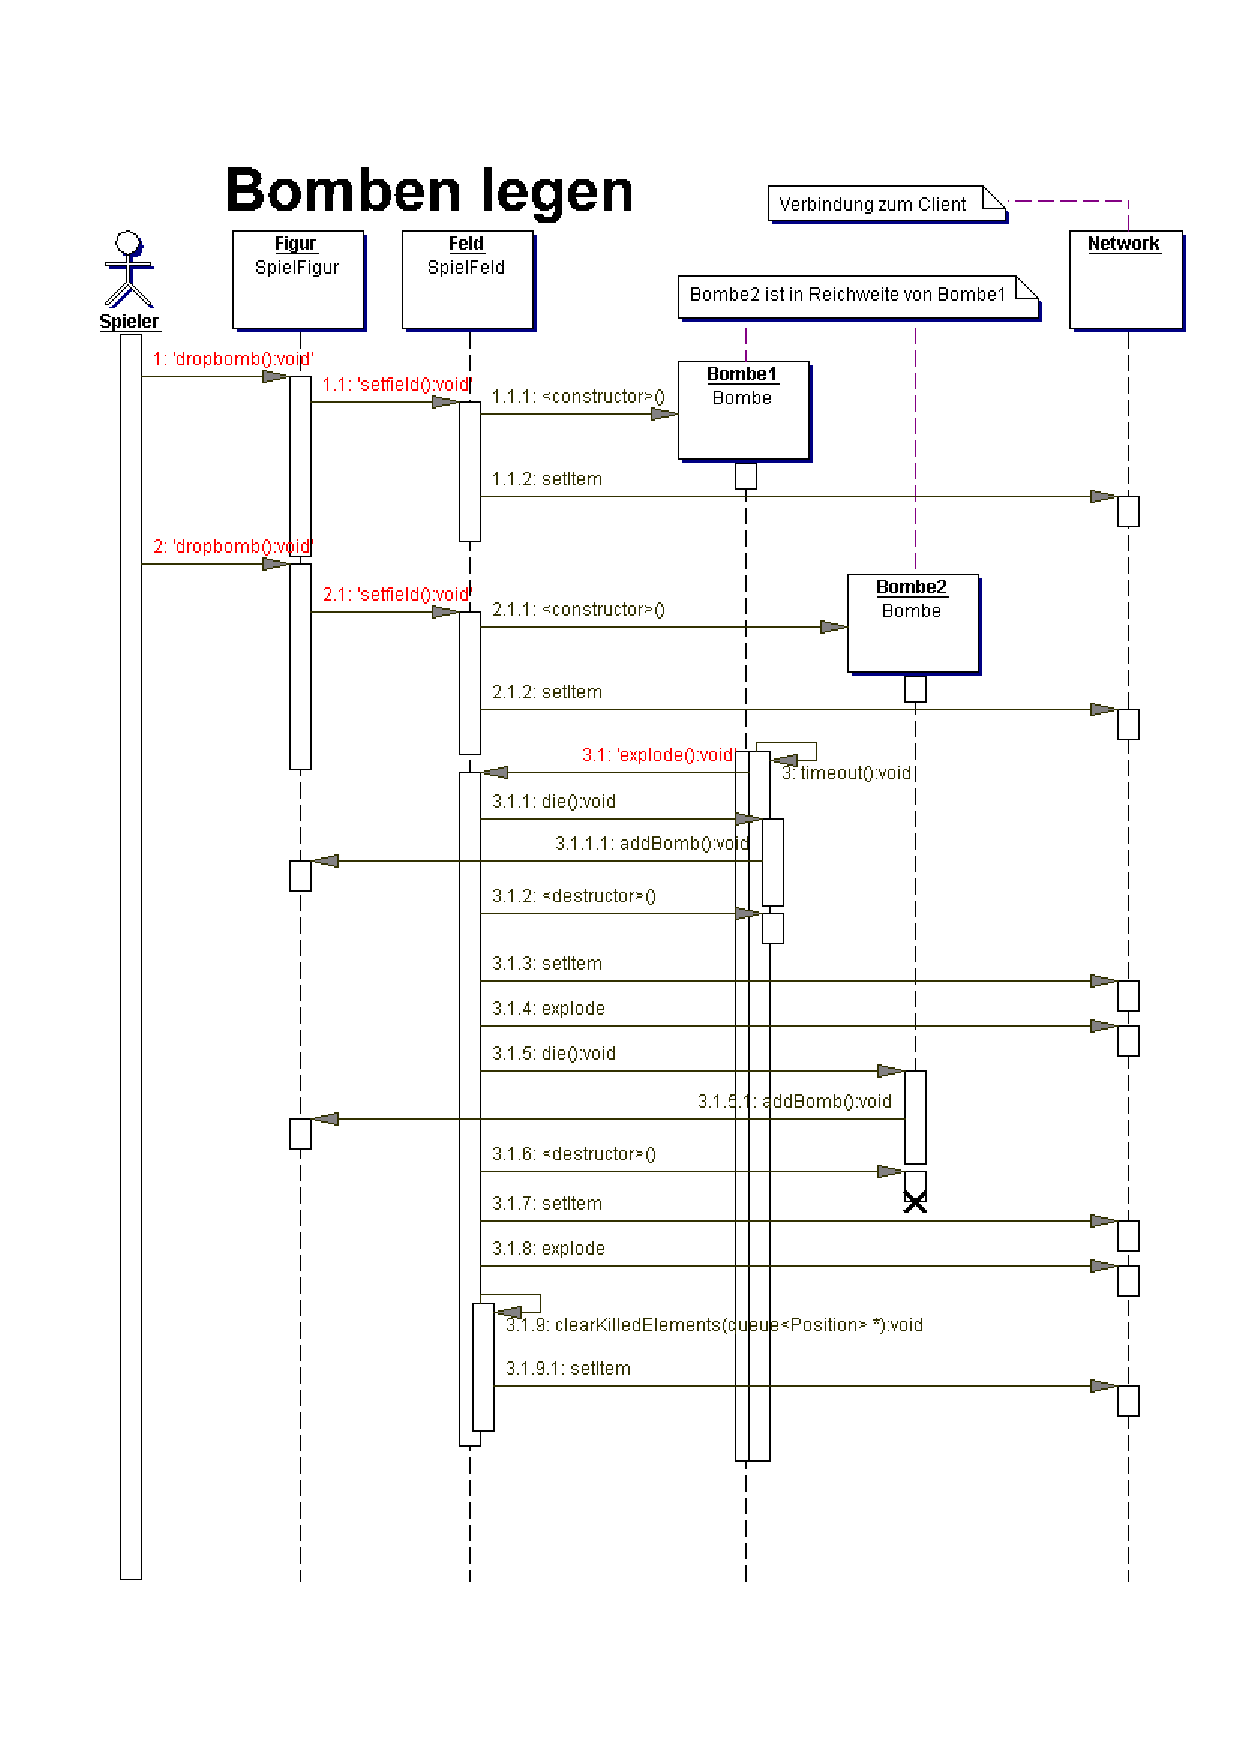
\includegraphics[height=18cm]{./images/bombenlegen.pdf}}
  \end{center}
  \caption{Sequenzdiagramm f"ur das Legen von Bomben}
\end{figure}

% ProblemDomain  Klassenbeschrieb
% 19.4.2002 U.Heimann   Dokument erstellt
% 26.4.2002 U.Heimann   erweitert, korrigiert
%  2.5.2002 U.Heimann   �nderung Client/Server
%  5.6.2002 u.Heimann   �nderung Iteration 2
% 12.7.2002 U.Heimann   Endversion

\section{PD Klassenbeschreibung}
Die endg"ultige Version des Spiels soll "uber ein Netzwerk gespielt werden. Deshalb wird die PD in Server und Client unterteilt.
Die Klassen des Servers sind f"ur die Berechnung des gesamten Spielverlaufs (Positionen, Treffererkennung, ...) verantwortlich.
Der Client konvertiert die Steuerbefehle und schickt sie "uber das Netzwerk an den Server. Der Server berechnet die Auswirkungen
und schickt die "Anderungen zur"uck an alle Clients. Der Client reicht die "Anderungen wiederum an das User Interface weiter.
Jeder Spieler hat auf seinem Rechner eine Instanz des Clients, aber nur einer hat zus"atzlich noch eine Instanz des Servers.

\subsection{Klasse SpielManager}
Der Spielmanager ist f"ur die Verwaltung des Spiels verantwortlich. Er kontrolliert den Verbindungsaufbau
und -abbruch der Clients und erzeugt die zum Spielen notwendigen Objekte.
\subsubsection{Attribute}
\begin{tabular}{p{50mm}p{90mm}}
-serverGame      : bool           &  True wenn dieser PC als Server agiert. \\
-playerConnected : bool[]         &  True wenn mit der entsprechenden ID ein Spieler verbunden ist. \\
-playerName      : string[]       &  Namen der verbundenen Spieler. \\
-playerReady     : bool[]         &  True wenn der Spieler zum Spielen bereit ist. \\
-game            : Spiel*         &  Pointer auf das Spiel-Objekt. \\
-serverThread    : ServerThread*  &  Pointer auf Server-Listening-Thread. \\
-pdMutex         : QMutex*        &  Mutex zum Schutz der PD vor Mehrfachzugriff. \\
-serverMutex     : QMutex*        &  Mutex zum Beenden des Server-Threads. \\
-client          : Client*        &  Pointer auf Client-Objekt, zum Abfragen des Sockets. \\
-clientTimer     : QTimer*        &  Timer zur regelm"assigen Abfrage des Client-Sockets. \\
 & \\
-guiInputInterface      : GUIToPDInterface*  &  Interface  GUI $\rightarrow$ PD \\
-guiOutputInterface     : PDToGUIInterface*  &  Interface  PD  $\rightarrow$ GUI \\
-netInputInterface      : PDKontroller*      &  Interface  NET $\rightarrow$ PD \\
-netOutClientInterface  : ClientInterface*   &  Interface  PD (client) $\rightarrow$ NET \\
-netOutServerInterface  : ServerInterface*   &  Interface  PD (server) $\rightarrow$ NET \\

\end{tabular}
\subsubsection{Funktionen}
\begin{tabular}{p{50mm}p{90mm}}
+startServer(string playerName)        : void  &  Startet den Netzwerk-Server und meldet sich als Spieler an. \\
+joinServer(string ipAddress, string playerName)  : void  &  Startet den Netzwerk-Client und meldet sich beim Server an. \\
+startGame()                           : void  &  Initialisiert und startet das Spiel mit den verbundenen Spielern. \\
+endGame()                             : void  &  Beendet das laufende Spiel. \\
+killGame()                            : void  &  Bricht das laufende Spiel ab. (zu irgendeinem Zeitpunkt) \\
+errorMsg(int msgNr, string addInfo)   : void  &  Bearbeitet Fehlermeldungen vom Netzwerk. \\
 & \\
+newPlayer(int playerID, string playerName) : void  &  Ein neuer Spieler hat sich beim Server angemeldet. \\
+removePlayer(int playerID)            : void  &  Entfernt einen Spieler aus der Spielerliste und entfernt ihn aus dem Spiel. \\
+ready(int playerID)                   : void  &  Setzt den Spieler spielbereit. \\
+distributeMsg(string info)            : void  &  Schickt eine Nachricht an alle verbundenen Clients weiter. \\
 & \\
+connectConfirm()                      : void  &  Best"atigt die Verbindung zum Server. \\
+setPlayerName(int playerID, string name) : void &  Setzt den Namen eines Verbundenen Spielers. \\
+disconnect()                          : void  &  Meldet sich beim Server ab. \\
+run()                                 : void  &  Synchronisiert und startet das Spiel. \\
+infoMsg(string info)                  : void  &  Zeigt eine Nachricht vom Server an. \\
 & \\
-createNetworkServer()                 : void  &  Startet den Server-Listening-Thread. \\
-killNetworkServer()                   : void  &  Beendet den Server-Listening-Thread. \\
-createNetworkClient()                 : void  &  Startet den Client-Timer zur Abfrage des Sockets. \\
-killNetworkClient()                   : void  &  Beendet den Client-Timer. \\
 & \\
-clientTimeout()                       : void  &  wird bei Ablauf des Client-Timers aufgerufen. \\
\end{tabular}


\subsection{Klasse Spiel}
Die Klasse Spiel erzeugt die restliche Spielstruktur (Spielfeld, Spielfiguren) je nach Anzahl
Spieler. Es wird immer ein Client erstellt, und beim Spielf"uhrer zus"atzlich noch ein Server. Sie ist daf"ur verantwortlich,
dass das Spiel mit allen Clients synchronisiert ist bevor das Spiel gestartet wird. \\
\subsubsection{Attribute}
\begin{tabular}{p{50mm}p{90mm}}
-serverFeld  :  Spielfeld*         &  Pointer auf das ServerSpielfeld. \\
-figur[4]    :  Spielfigur*        &  Pointer auf die Spielfiguren des Servers. \\
-clientFeld  :  SpielfeldClient*   &  Pointer auf das ServerSpielfeld. \\
-spieler     :  SpielerClient*     &  Pointer auf die Spielfigur des Clients. \\
\end{tabular}

\subsubsection{Funktionen}
\begin{tabular}{p{50mm}p{90mm}}
+initClient()             : void  &  Initialisiert die Client-Umgebung. \\
+initServer(bool activPlayers[], string playerNames[]) : void  &  Initialisiert die Server-Umgebung. \\
+ready()                  : bool  &  gibt TRUE zur"uck wenn Client bereit ist. \\
+run()                    : void  &  Synchronisiert und startet das Spiel. \\
+killPlayer(int playerID) : void  &  Entfernt einen Spieler vom Spielfeld. \\
-destroyClient()          : void  &  R"aumt die Client-Umgebung nach Spielende auf. \\
-destroyServer()          : void  &  R"aumt die Server-Umgebung nach Spielende auf. \\
\end{tabular}


\subsection{Klasse GUIToPDInterface (Singleton)}
"Uber diese Schnittstelle sendet das User Interface die Tastatureingaben des Spielers an die PD.\\
\subsubsection{Attribute}
\begin{tabular}{p{50mm}p{90mm}}
-manager : SpielManager*   &  Pointer auf den Spielmanager. \\
-spieler : SpielerClient*  &  Pointer auf den Spieler. \\
-pdMutex : QMutex*         &  Sichert die PD vor Mehrfachzugriff ab. \\
\end{tabular}
\subsubsection{Funktionen}
\begin{tabular}{p{50mm}p{90mm}}
+setManager(SpielManager* man, QMutex* pdMut) : void  &  Registriert den Spielmanager. \\
+setPlayer(SpielerClient* player): void  &  Registriert den Spieler. \\
+startServer(const char* player) : void  &  Startet neues Spiel als Server. \\
+joinServer(const char* ipAdress, const char* playerName) : void  &  Startet neues Spiel als Client. \\
+startGame()                     : void  &  Startet das Spiel mit den verbundenen Spielern (nur Server) \\
+killGame()                      : void  &  Beendet das Spiel zu einem beliebigen Zeitpunkt. \\
+keyPressed(int key)             : void  &  Eine Taste wurde gedr"uckt. \\
+keyReleased(int key)            : void  &  Eine Taste wurde losgelassen. \\
\end{tabular}

\subsection{Klasse PDToGUIInterface (Singleton)}
"Uber diese Schnittstelle sendet die PD die "Anderungen des Spielfeldes an das User Interface.
(siehe GUI) \\

\subsection{Klasse ServerInterface}
(siehe Netzwerk)

\subsection{Klasse ClientInterface}
(siehe Netzwerk)

\subsection{Klasse ServerThread}
Separater Thread f"ur die Abfrage des Server-Sockets. (Abgeleitet von QThread) \\
\subsubsection{Attribute}
\begin{tabular}{p{50mm}p{90mm}}
-runServer : QMutex*  &  Synchronisationsobjekt zum Beenden des Serverthreads. \\
-pdMutex   : QMutex*  &  Sichert die PD vor Mehrfachzugriff ab. \\
\end{tabular}
\subsubsection{Funktionen}
\begin{tabular}{p{50mm}p{90mm}}
+run()     : void     &  Ausf"uhrungsroutine des Threads. \\
\end{tabular}

\subsection{Klasse PDKontroller (Singleton)}
Der PDKontroller empf"angt und verarbeitet die Nachrichten vom Netzwerk. Sie ist als Singleton realisert und ist die Schnittstelle
vom Netzwerk zu der PD.
\subsubsection{Attribute}
\begin{tabular}{p{50mm}p{90mm}}
-spielManager : SpielManager*     &  Pointer auf den Manager. \\
-serverFigur  : Spielfigur*[]    &  Pointer auf die Spielfiguren (nur Server) \\
-clientFeld   : SpielfeldClient*  &  Pointer auf das Spielfeld. \\
\end{tabular}
\subsubsection{Funktionen}
\begin{tabular}{p{50mm}p{90mm}}
+setManager(SpielManager* manager) : void  &  Registriert den Spielmanager. \\
+setSpielfigur(int playerID, Spielfigur* figur) : void  &  Registriert eine Spielfigur. \\
+setClientFeld(SpielfeldClient* feld) : void  &  Registriert das Spielfeld. \\
Manager-Funktionen & \\
+newPlayer(int playerID, string playerName) : void  &  Ein neuer Spieler hat sich beim Server angemeldet. \\
+disconnect(int playerID)              : void  &  Ein Spieler hat sich abgemeldet. \\
+disconnect()                          : void  &  Der Server hat sich abgemeldet. \\
+ready(int playerID)                   : void  &  Der Spieler ist spielbereit. \\
+run()                                 : void  &  Spielstart  \\
+endGame()                             : void  &  Beendet das Spiel. \\
+connectConfirm()                      : void  &  Best"atigt die Verbindung zum Server. \\
+receiveMsg(string msg)                : void  &  Empf"angt eine Nachricht vom Server. \\
+receiveMsg(int playerID, string msg)  : void  &  Empf"angt eine Nachricht vom Client (zum Verteilen an alle Clients). \\
+errorMsg(int msgNumber, string addInfo) : void  & Empf"angt eine Fehlermeldung vom Netzwerk. \\
+setPlayerName(int playerID, string name) :  &  Setzt den Namen eines Spielers. \\
Server-Funktionen & \\
+setDirection(int direction, int playerID) : void  &  Setzt neue Laufrichtung des Spielers. \\
+setBombPressed(bool keypressed, int playerID) : void   &  Setzt das Bomben-lege-Flag. \\
Client-Funtionen & \\
+setPlayfield(vector<int> feldinfo, int zeilenbreite) : void  &  Initialisiert das ganze Spielfeld. \\
+setItem(Position position, int item) : void  &  Setzt ein einzelnes Objekt auf dem Spielfeld. \\
+setPlayer(int playerID, Position position) : void  &  Setzt die Position einer Spielfigur. \\
+delPlayer(int playerID) : void  &  L"oscht einen Spieler vom Spielfeld. \\
+explode(Position position, int reichweite) : void  &  L"ost eine Explosion auf dem Spielfeld aus. \\
\end{tabular}


\subsection{Klasse Spielfeld}
Die Klasse Spielfeld enth"alt ein Array das den aktuellen Zustand und die Positionen aller Spielelemente representiert. Sie hat
Zugriff auf alle spielentscheidenden Informationen. \\
\subsubsection{Attribute}
\begin{tabular}{p{50mm}p{90mm}}
-feld         : Spielelement*[]         &  Abbild des aktuellen Spielstandes. Jeder Eintrag im Array entspricht einem Feld. d.h.
                                           es k"onnen nicht mehrere Elemente auf einem Feld sein. (Spielfiguren werden hier
                                           nicht gespeichert!) \\
-player       : Spielfigur[]            &  Zeigerliste auf alle Spielfiguren des aktuellen Spiels. Die Position der Figur ist
                                           bei der Figur gespeichert.\\
-game         : Spiel*                  &  Pointer auf das Spiel-Objekt. \\
-netInterface : ServerInterface*        &  Pointer zum Netzwerk-Interface des Servers. \\
-minPlayers   : int                     &  Sind weniger Spieler als minPlayers auf dem Feld wird das Spiel beendet. \\
\end{tabular}
\subsubsection{Funktionen}
\begin{tabular}{p{50mm}p{90mm}}
+startGame() : void  &  Startet das Spiel. \\
+stopGame() : void  &  Beendet das Spiel. \\
+setField(Position pos, int item, Spielfigur* figur = NULL) : void  &  Setzt ein bestimmtes Element an die Koordinate (x,y). \\
+getField(Position pos) : int item        &  Liefert das Element das sich an der Koordinate (x,y) befindet. \\
+setPlayer(int playerID, Spielfigur* player) : void     &  Meldet einen neuen Spielfigur beim Spielfeld an. \\
+delPlayer(int playerID) : void  &  Meldet den Spieler ab. \\
+explode(Position pos, int reichweite, queue<Position>* toDie = NULL) : void  &  Berechnet die Explosion. \\
-clearKilledElements(queue$<$Position$>$* toDie) : void  &  L"oscht die gesprengten Elemente vom Spielfeld. \\
\end{tabular}

\subsection{Klasse Spielfigur}
Die Klasse Spielfigur enth"alt alle wichtigen Informationen "uber Position und Zustand der Spielfigur. \\
\subsubsection{Attribute}
\begin{tabular}{p{50mm}p{90mm}}
-spielfeld     : Spielfeld*       &  Pointer auf das Spielfeld-Objekt. \\
-pdKontroller  : PDKontroller*    &  Pointer auf den den PD-Kontroller. F"ur ankommende Meldungen vom Netzwerk. \\
-netInterface  : ServerInterface* &  Pointer auf das Netzwerk-Interface. F"ur abgehende Meldungen ans Netzwerk. \\

-playerID      : int       &  Spielernummer  \\
-playerName    : string    &  Name des Spielers. \\
-position      : Position  &  Position der Spielfigur auf dem Spielfeld in (x,y) Koordinaten. \\
-direction     : int       &  Richtung in die die Spielfigur gehen m"ochte. (STAY, UP, DOWN, LEFT, RIGHT) \\
-numberOfBombs : int       &  Die Anzahl Bomben die er noch legen darf. -1 wenn Bombe gelegt wurde, +1 wenn seine Bombe explodiert ist
                              oder ein Bomben-Powerup aufgenommen wurde. \\
-reichweite    : int       &  Reichweite der Bombe in Feldern. Wird der Bombe "ubergeben wenn sie gelegt wird. Wird erh"oht, wenn ein
                              Flammen-Powerup aufgenommen wird. \\
-alive         : bool      &  TRUE wenn die Spielfigur noch lebt. \\
-bombPressed   : bool      &  TRUE wenn die Bomben-lege-Taste gedr"uckt ist. \\
-moveTimer     : QTimer*   &  Timer f"ur die Bewegungs-Verz"ogerung. \\
\end{tabular}
\subsubsection{Funktionen}
\begin{tabular}{p{50mm}p{90mm}}
+setDirection(int dir)          : void   &  Setzt die Laufrichtung der Spielfigur (STAY, UP, DOWN, LEFT, RIGHT). \\
+setBombPressed(bool bomb)      : void   &  Setzt das bombPressd Flag (bomben-lege-Taste gedr"uckt). \\
+getName()                      : string &  Liefert den Namen des Spielers. \\
+getPosition()                : Position &  Liefert die aktuelle Position der Spielfigur. \\
+addBomb()                      : void   &  F"ugt eine Bombe zum Arsenal der Spielfigur hinzu. \\
+wakeup()                       : void   &  Erweckt die Spielfigur zum Leben, erlaubt ihr sich zu bewegen. \\
+die()                          : void   &  Zerst"ort die Spielfigur wenn sie gesprengt wurde. \\
+move()                         : bool   &  Bewegt die Spielfigur um ein Feld in die aktuelle Richtung (direction). \\
+getReichweite()                : int    &  Gibt die Reichweite zur"uck. \\
-dropBomb()                     : void   &  Legt eine Bombe an der aktuellen Position sofern noch Bomben im Arsenal. \\
-checkField(int posx, int posy) : int    &  Pr"uft ob ein Feld auf dem Spielfeld passierbar ist oder nicht. \\
-timerDone()                    : void   &  Wird aufgerufen wenn der moveTimer abgelaufen ist. \\
\end{tabular}

\subsection{Klasse SpielerClient}
Die Klasse Spieler empf"angt die Benutzereingaben, bestimmt die daraus folgenden Aktionen und leitet sie an den Server weiter.\\
\subsubsection{Attribute}
\begin{tabular}{p{50mm}p{90mm}}
-guiInterface : GUIToPDInterface*  &  Pointer zum GUI-Interface, zum Empfang der Benutzereingaben. \\
-netInterface : ClientInterface*   &  Pointer zum Netzwerk-Interface, zum Versenden der Aktionen. \\
-keylist      : bool[5]            &  Speichert die Informationen welche Tasten momentan gedr"uckt sind. \\
-oldDirection : int                &  Die zuletzt "ubermittelte bewegungsrichtung. \\
\end{tabular}
\subsubsection{Funktionen}
\begin{tabular}{p{50mm}p{90mm}}
+keyPressed(int key) : void      &  Eine Taste wurde gedr"uckt. \\
+keyReleased(int key) : void     &  Eine Taste wurde losgelassen. \\
-computeDirection() : void       &  Berechnet die Laufrichtung aus den Daten der keylist und sendet sie an den Server. \\
\end{tabular}

\subsection{Klasse SpielfeldClient}
Die Klasse SpielfeldClient hat ein vereinfachtes Abbild der Spielsituation gespeichert. Sie ben"otigt dieses zur
berechnung der Explosionen. Sie empf"angt alle "Anderungen vom Server und gibt sie ans GUI weiter.\\
\subsubsection{Attribute}
\begin{tabular}{p{50mm}p{90mm}}
-guiInterface   : PDToGUIInterface*  &  Pointer zum GUI-Interface, zum Senden der "Anderungen. \\
-pdKontroller   : PDKontroller*      &  Pointer zum PD-Kontroller, zum Empfangen der Spielfeld"anderungen. \\
-field          : int[][]            &  Vereinfachtes Abbild der Spielsituation. \\
-playerPosition : Position[4]        &  Die Positionen der Spieler auf dem Spielfeld. \\
-readySet       : bool               &  TRUE wenn bereit zum spielen. \\
\end{tabular}
\subsubsection{Funktionen}
\begin{tabular}{p{50mm}p{90mm}}
+setPlayfield(vector<int> feldinfo, int zeilenbreite) :  void  &  Setzt das gesamte Spielfeld. \\
+setField(Position pos, int item)       : void  &  Setzt ein bestimmtes Element an die Koordinate (x,y). \\
+setPlayer(int playerID, Position pos)  : void  &  Setzt die Spielfigur (nr) an die Position (x,y). \\
+delPlayer(int playerID)                : void  &  L"oscht einen Spieler vom Spielfeld. \\
+explode(Position pos, int reichweite)  : void  &  berechnet eine Explosion. \\
\end{tabular}

\subsection{Klasse SpielElement}
Oberklasse aller auf dem Spielfeld platzierbaren Elemente wie Mauer, Wand, Bombe und Powerup (ausser den Spielfiguren). \\
\subsubsection{Attribute}
\begin{tabular}{p{50mm}p{90mm}}
-position    : Position  &  Position des Elements. \\
-elementType : int       &  Typ des Elements. \\
\end{tabular}
\subsubsection{Funktionen}
\begin{tabular}{p{50mm}p{90mm}}
+die()     : SpielElement*  &  Rein Virtuelle Funktion die beim sprengen des Objekts aufgerufen wird. \\
+getType() : int            &  Liefert den Typ des Elements. \\
\end{tabular}

\subsection{Klasse Mauer}
Die Mauer ist vom Spielelement abgeleitet. Sie kann durch eine Explosion nicht zerst"ort werden. Sie hat keine
spezielle Funktionalit"at.\\

\subsection{Klasse Wand}
Die Wand ist vom Spielelement abgeleitet. Sie kann durch eine Explosion zerst"ort werden und erzeugt dabei ev. ein Powerup. \\
\subsubsection{Attribute}
\begin{tabular}{p{50mm}p{90mm}}
-powerupType : int  &  Typ des versteckten Powerups. \\
\end{tabular}
\subsubsection{Funktionen}
\begin{tabular}{p{50mm}p{90mm}}
+getPowerupType() : int  &  Liefert den Typ des versteckten Powerups. \\
\end{tabular}

\subsection{Klasse Bombe}
Die Bombe ist vom Spielelement abgeleitet. Beim Erzeugen startet der Timer, der am Ende eine Explosion und damit
die Zerst"orung der Bombe einleitet. Sie kann durch eine Explosion zerst"ort werden und explodiert dabei selbst. \\
\subsubsection{Attribute}
\begin{tabular}{p{50mm}p{90mm}}
-dropper      : Spielfigur*  &  Pointer auf die Spielfigur die sie erzeugt hat. \\
-playfield    : Spielfeld*   &  Pointer auf das Spielfeld auf dem sie liegt. \\
-explodeTimer : QTimer*      &  Timer zur Verz"ogerung der Explosion. \\
-reichweite   : int          &  Die Reichweite der Explosion, wird beim Erzeugen gesetzt. \\
\end{tabular}
\subsubsection{Funktionen}
\begin{tabular}{p{50mm}p{90mm}}
+getReichweite() : int   &  Liefert die Reichweite der Bombe. \\
-timeout()       : void  &  wird vom Timer aufgerufen wenn er abgelaufen ist. L"ost die Explosion aus. \\
\end{tabular}

